        %%******************************************%%
        %%                                          %%
        %%        Modello di tesi di laurea         %%
        %%            di Andrea Giraldin            %%
        %%                                          %%
        %%             2 novembre 2012              %%
        %%                                          %%
        %%******************************************%%


% I seguenti commenti speciali impostano:
% 1. 
% 2. PDFLaTeX come motore di composizione;
% 3. tesi.tex come documento principale;
% 4. il controllo ortografico italiano per l'editor.

% !TEX encoding = UTF-8
% !TEX TS-program = pdflatex
% !TEX root = tesi.tex
% !TEX spellcheck = it-IT

% PDF/A filecontents
\RequirePackage{filecontents}
\begin{filecontents*}{\jobname.xmpdata}
  \Title{Document’s title}
  \Author{Author’s name}
  \Language{it-IT}
  \Subject{The abstract, or short description.}
  \Keywords{keyword1\sep keyword2\sep keyword3}
\end{filecontents*}

\documentclass[12pt,                    % corpo del font principale
               a4paper,                 % carta A4
               twoside,                 % impagina per fronte-retro
               openright,               % inizio capitoli a destra
               english,                 
               italian,                 
               ]{book}    

\linespread{1.5} 
\usepackage[a4paper, top=3cm, bottom=3cm, left=3cm, right=3cm]{geometry}
%\documentclass[12pt]{article}
%\usepackage[a4paper, top=3cm, bottom=3cm, left=3cm, right=3cm]{geometry}
%\geometry{a4paper, top=3cm, bottom=3cm, left=3cm, right=3cm}
%\linespread{1.5}

%\documentclass[12pt]{article}
%\usepackage[a4paper, margin=2cm]{geometry}
%\linespread{1.5}

%**************************************************************
% Importazione package
%************************************************************** 

\PassOptionsToPackage{dvipsnames}{xcolor} % colori PDF/A

\usepackage{colorprofiles}

\usepackage[a-2b,mathxmp]{pdfx}[2018/12/22]
                                        % configurazione PDF/A
                                        % validare in https://www.pdf-online.com/osa/validate.aspx

%\usepackage{amsmath,amssymb,amsthm}    % matematica

\usepackage[T1]{fontenc}                % codifica dei font:
                                        % NOTA BENE! richiede una distribuzione *completa* di LaTeX

\usepackage[utf8]{inputenc}             % codifica di input; anche [latin1] va bene
                                        % NOTA BENE! va accordata con le preferenze dell'editor

\usepackage[english, italian]{babel}    % per scrivere in italiano e in inglese;
                                        % l'ultima lingua (l'italiano) risulta predefinita

\usepackage{bookmark}                   % segnalibri

\usepackage{caption}                    % didascalie

\usepackage{chngpage,calc}              % centra il frontespizio

\usepackage{csquotes}                   % gestisce automaticamente i caratteri (")

\usepackage{emptypage}                  % pagine vuote senza testatina e piede di pagina

\usepackage{epigraph}			% per epigrafi

\usepackage{eurosym}                    % simbolo dell'euro

%\usepackage{indentfirst}               % rientra il primo paragrafo di ogni sezione

\usepackage{graphicx}                   % immagini

\usepackage{hyperref}                   % collegamenti ipertestuali

\usepackage[binding=5mm]{layaureo}      % margini ottimizzati per l'A4; rilegatura di 5 mm

\usepackage{listings}                   % codici

\usepackage{microtype}                  % microtipografia

\usepackage{mparhack,fixltx2e,relsize}  % finezze tipografiche

\usepackage{nameref}                    % visualizza nome dei riferimenti                                      
\usepackage[font=small]{quoting}        % citazioni

\usepackage{subfig}                     % sottofigure, sottotabelle

\usepackage[italian]{varioref}          % riferimenti completi della pagina

\usepackage{booktabs}                   % tabelle                                       
\usepackage{tabularx}                   % tabelle di larghezza prefissata                                    
\usepackage{longtable}                  % tabelle su più pagine                                        
\usepackage{ltxtable}                   % tabelle su più pagine e adattabili in larghezza

\usepackage[toc, acronym]{glossaries}   % glossario
                                        % per includerlo nel documento bisogna:
                                        % 1. compilare una prima volta tesi.tex;
                                        % 2. eseguire: makeindex -s tesi.ist -t tesi.glg -o tesi.gls tesi.glo
                                        % 3. eseguire: makeindex -s tesi.ist -t tesi.alg -o tesi.acr tesi.acn
                                        % 4. compilare due volte tesi.tex.

\usepackage[backend=biber,style=verbose-ibid,hyperref,backref]{biblatex}
                                        % eccellente pacchetto per la bibliografia; 
                                        % produce uno stile di citazione autore-anno; 
                                        % lo stile "numeric-comp" produce riferimenti numerici
                                        % per includerlo nel documento bisogna:
                                        % 1. compilare una prima volta tesi.tex;
                                        % 2. eseguire: biber tesi
                                        % 3. compilare ancora tesi.tex.

%**************************************************************
% file contenente le impostazioni della tesi
%**************************************************************

%**************************************************************
% Frontespizio
%**************************************************************

% Autore
\newcommand{\myName}{Gabriel Bizzo}                                    
\newcommand{\myTitle}{Distorsione: implementazione di un processore di segnale audio digitale per la ricerca e lo studio del fenomeno}

% Extra                
\newcommand{\DCPL}{DCPL: 34}
\newcommand{\DCSL}{DCSL: 34}

% Tipo di tesi                   
\newcommand{\myDegree}{Tesi di diploma accademico di I livello}

% Università             
\newcommand{\myUni}{Conservatorio Cesare Pollini}

% Facoltà       
\newcommand{\myFaculty}{Tesi di diploma accademico di I livello in Musica Elettronica indirizzo tecnico di sala di registrazione}

% Dipartimento
\newcommand{\myDepartment}{Dipartimento di Musica Elettronica}

% Titolo del relatore
\newcommand{\profTitle}{Prof. }

% Relatore
\newcommand{\myProf}{Julian Scordato}

% Luogo
\newcommand{\myLocation}{Padova}

% Anno accademico
\newcommand{\myAA}{2020-2021}

% Data discussione
\newcommand{\myTime}{Novembre 2021}


%**************************************************************
% Impostazioni di impaginazione
% see: http://wwwcdf.pd.infn.it/AppuntiLinux/a2547.htm
%**************************************************************

\setlength{\parindent}{14pt}   % larghezza rientro della prima riga
\setlength{\parskip}{0pt}   % distanza tra i paragrafi


%**************************************************************
% Impostazioni di biblatex
%**************************************************************
\bibliography{bibliografia} % database di biblatex 

\defbibheading{bibliography} {
    \cleardoublepage
    \phantomsection 
    \addcontentsline{toc}{chapter}{\bibname}
    \chapter*{\bibname\markboth{\bibname}{\bibname}}
}

\setlength\bibitemsep{1.5\itemsep} % spazio tra entry

\DeclareBibliographyCategory{opere}
\DeclareBibliographyCategory{web}

\addtocategory{opere}{womak:lean-thinking}
\addtocategory{web}{site:agile-manifesto}

\defbibheading{opere}{\section*{Riferimenti bibliografici}}
\defbibheading{web}{\section*{Siti Web consultati}}


%**************************************************************
% Impostazioni di caption
%**************************************************************
\captionsetup{
    tableposition=top,
    figureposition=bottom,
    font=small,
    format=hang,
    labelfont=bf
}

%**************************************************************
% Impostazioni di glossaries
%**************************************************************

%**************************************************************
% Acronimi
%**************************************************************
\renewcommand{\acronymname}{Acronimi e abbreviazioni}

\newacronym[description={\glslink{apig}{Application Program Interface}}]
    {api}{API}{Application Program Interface}

\newacronym[description={\glslink{umlg}{Unified Modeling Language}}]
    {uml}{UML}{Unified Modeling Language}
    
\newacronym[description={\glslink{dimg}{Distorsione di intermodulazione}}]
    {dim}{DIM}{Distorsione di intermodulazione}
    
\newacronym[description={\glslink{dbfsg}{Decibel Full Scale}}]
    {dbfs}{dBFS}{Decibel Full Scale}
    
\newacronym[description={\glslink{iirg}{Infinite Impulse Response}}]
    {iir}{IIR}{Infinite Impulse Response}
    
\newacronym[description={\glslink{lfog}{Low Frequency Oscillator}}]
    {lfo}{LFO}{Low Frequency Oscillator}
    
\newacronym[description={\glslink{dawg}{Digital Audio Workstation}}]
    {daw}{DAW}{Digital Audio Workstation}
    
\newacronym[description={\glslink{fftg}{Fast Fourier Transform}}]
    {fft}{FFT}{Fast Fourier Transform}

%**************************************************************
% Glossario
%**************************************************************
%\renewcommand{\glossaryname}{Glossario}

\newglossaryentry{apig}
{
    name=\glslink{api}{API},
    text=Application Program Interface,
    sort=api,
    description={in informatica con il termine \emph{Application Programming Interface API} (ing. interfaccia di programmazione di un'applicazione) si indica ogni insieme di procedure disponibili al programmatore, di solito raggruppate a formare un set di strumenti specifici per l'espletamento di un determinato compito all'interno di un certo programma. La finalità è ottenere un'astrazione, di solito tra l'hardware e il programmatore o tra software a basso e quello ad alto livello semplificando così il lavoro di programmazione}
}

\newglossaryentry{umlg}
{
    name=\glslink{uml}{UML},
    text=UML,
    sort=uml,
    description={in ingegneria del software \emph{UML, Unified Modeling Language} (ing. linguaggio di modellazione unificato) è un linguaggio di modellazione e specifica basato sul paradigma object-oriented. L'\emph{UML} svolge un'importantissima funzione di ``lingua franca'' nella comunità della progettazione e programmazione a oggetti. Gran parte della letteratura di settore usa tale linguaggio per descrivere soluzioni analitiche e progettuali in modo sintetico e comprensibile a un vasto pubblico}
}

\newglossaryentry{dimg}
{
    name=\glslink{dim}{DIM},
    text=DIM,
    sort=dim,
    description={\emph{La distorsione di intermodulazione} consiste nella modulazione di ampiezza di segnali contenenti due o più frequenze diverse, causata principalmente dalla non linearità di un sistema. L'intermodulazione tra i componenti di frequenza forma componenti aggiuntivi a frequenze che non sono solo alle frequenze armoniche (multipli interi) di entrambi, come la distorsione armonica, ma anche alle frequenze somma e differenza delle frequenze originali e alle somme e differenze di multipli di quelle frequenze}
}

\newglossaryentry{dbfsg}
{
    name=\glslink{dbfs}{dBFS},
    text=dBFS,
    sort=dbfs,
    description={I \emph{Decibel Full Scale} (dBFS o dB FS) sono un'unità di misura per i livelli di ampiezza nei sistemi digitali che hanno un livello di picco massimo definito. Il livello di 0dBFS è assegnato al massimo livello digitale possibile. Ad esempio, un segnale che raggiunge il 50\% del livello massimo ha un livello di -6dBFS, che è 6dB al di sotto del massimo della scala}
}

\newglossaryentry{pre-enfasig}
{
    name=Pre-enfasi,
    text=pre-enfasi,
    sort=preenfasi,
    description={La \textit{Pre-Enfasi} di un segnale audio consiste in un processo in cui è previsto l'utilizzo di due shelf filter. Entrambi i filtri possono essere o high shelf o low shelf e sono posti uno prima e uno dopo un ulteriore blocco di elaborazione audio (spesso consiste in un effetto di distorsione). L'operazione di pre-enfasi prevede l'applicazione di un'attenuazione o enfatizazione della frequenza del primo filtro, in modo tale da effettuare l'operazione inversa nel secondo filtro}
}

\newglossaryentry{opensourceg}
{
    name=Open-source,
    text=open-source,
    sort=opensource,
    description={Con \textit{open-source} (in italiano sorgente aperto), in informatica, si indica un tipo di software o il suo modello di sviluppo o distribuzione. Un software open source è reso tale per mezzo di una licenza attraverso cui i detentori dei diritti favoriscono la modifica, lo studio, l’utilizzo e la redistribuzione del codice sorgente}
}

\newglossaryentry{iirg}
{
    name=\glslink{iir}{IIR},
    text=IIR,
    sort=iir,
    description={In teoria dei segnali, un sistema dinamico \textit{Infinite Impulse Response} (in italiano risposta all'impulso infinita e spesso abbreviato in IIR) è un sistema dinamico causale la cui risposta impulsiva non è nulla al tendere all'infinito del tempo. I sistemi la cui risposta si annulla ad un tempo finito sono invece detti finite impulse response (FIR). Sebbene la definizione si adatti a sistemi tempo-continui, solitamente si ha a che fare con sistemi numerici, spesso i filtri digitali}
}

\newglossaryentry{lfog}
{
    name=\glslink{lfo}{LFO},
    text=LFO,
    sort=lfo,
    description={L'\textit{oscillatore a bassa frequenza} o LFO (sigla di Low Frequency Oscillator) è un generatore di forme d'onda a frequenza infrasonica, con funzione di modulatore di effetti, negli strumenti musicali elettronici. Per potersi considerare tale deve stare al di sotto di 20 Hz proprio perché l'orecchio umano può udire i suoni nell'intervallo dai 20 Hz ai 20 kHz e serve a modulare altri segnali}
}

\newglossaryentry{sidechaing}
{
    name=Sidechain,
    text=sidechain,
    sort=sidechain,
    description={Il \textit{sidechain} è una tecnica di compressione che, applicato a una traccia, attiva la compressione di un processore di dinamica a partire da un altro segnale audio esterno a tale traccia. Di norma i compressori vengono cablati in insert e il loro funzionamento dipende dal materiale audio che passa per quella data traccia. Se a un compressore posto in insert viene attivato il controllo sidechain, questo smetterà di funzionare, fin quando ad esso verrà indicato quale segnale dovrà fare da trigger (da azionatore)}
}

\newglossaryentry{dawg}
{
    name=\glslink{daw}{DAW},
    text=DAW,
    sort=daw,
    description={Una \textit{Workstation Audio Digitale}, a cui ci si riferisce spesso anche con il nome inglese di Digital Audio Workstation o con il suo acronimo DAW, è un sistema elettronico progettato per la registrazione, il montaggio e la riproduzione dell'audio digitale}
}

\newglossaryentry{powerchordg}
{
    name=Power Chord,
    text=power chord,
    sort=powerchord,
    description={Un \textit{power chord} (in inglese, letteralmente, "accordo potente"), anche noto come accordo di quinta o quinta vuota, è un bicordo i cui suoni vengono di solito eseguiti simultaneamente}
}

\newglossaryentry{pluging}
{
    name=Plugin,
    text=plugin,
    sort=plugin,
    description={Un \textit{plugin} in campo informatico corrisponde ad un programma non autonomo che interagisce con un altro programma per ampliarne o estenderne le funzionalità originarie (ad es. un plugin per un software di grafica permette l'utilizzo di nuove funzioni non presenti nel software principale): possono essere utilizzati non solo su software, ma anche su qualunque cosa che possa essere visitata da chiunque, quindi pubblica (ad es. i videogiochi online)}
}

\newglossaryentry{ditheringg}
{
    name=Dithering,
    text=dithering,
    sort=dithering,
    description={Il \textit{dithering}, nella elaborazione numerica di segnali, è una forma di rumore con una opportuna distribuzione, che viene volontariamente aggiunto ai campioni con l'obiettivo di minimizzare la distorsione introdotta dal troncamento nel caso in cui si riquantizzino i campioni stessi. Il dithering viene usato abitualmente nell'elaborazione di segnali video e audio campionati e quantizzati}
}

\newglossaryentry{mockupg}
{
    name=Mockup,
    text=mockup,
    sort=mockup,
    description={Un \textit{mockup}, o mock-up, è una realizzazione a scopo illustrativo o meramente espositivo di un oggetto o un sistema, senza le complete funzioni dell'originale; un mockup può rappresentare la totalità o solo una parte dell'originale di riferimento (già esistente o in fase di progetto), essere in scala reale oppure variata}
}

\newglossaryentry{fftg}
{
    name=\glslink{fft}{FFT},
    text=FFT,
    sort=fft,
    description={In matematica, la \textit{trasformata di Fourier veloce}, spesso abbreviata con FFT (dall'inglese Fast Fourier Transform), è un algoritmo ottimizzato per calcolare la trasformata discreta di Fourier (DFT) o la sua inversa. La FFT è utilizzata in una grande varietà di applicazioni, dall'elaborazione di segnali digitali alla soluzione di equazioni differenziali alle derivate parziali agli algoritmi per moltiplicare numeri interi di grandi dimensioni grazie al basso costo computazionale}
}

\newglossaryentry{polimorfismog}
{
    name=Polimorfismo,
    text=polimorfismo,
    sort=polimorfismo,
    description={In informatica, il termine \textit{polimorfismo} viene usato in senso generico per riferirsi a espressioni che possono rappresentare valori di diversi tipi (dette espressioni polimorfiche). In un linguaggio non tipizzato, tutte le espressioni sono intrinsecamente polimorfiche. Il termine nel contesto della programmazione orientata agli oggetti si riferisce al fatto che un'espressione il cui tipo sia descritto da una classe A può assumere valori di un qualunque tipo descritto da una classe B sottoclasse di A (polimorfismo per inclusione)}
}

\newglossaryentry{dspg}
{
    name=DSP,
    text=DSP,
    sort=dsp,
    description={Digital Signal Processing}
}

\newglossaryentry{projucerg}
{
    name=Projucer,
    text=Projucer,
    sort=projucer,
    description={\textit{Projucer} è uno strumento per la creazione e la gestione di progetti JUCE. Una volta specificati i file e le impostazioni per un progetto JUCE, Projucer genera automaticamente una raccolta di file di progetto di terze parti per consentire la compilazione nativa del progetto su ciascuna piattaforma di destinazione. Attualmente può generare progetti Xcode, Visual Studio, Linux Makefile, CodeBlocks e build Android Ant. Oltre a fornire un modo per gestire i file e le impostazioni di un progetto, ha anche un editor di codice, un editor GUI integrato, procedure guidate per la creazione di nuovi progetti/file e un motore di codifica live utile per la progettazione dell'interfaccia utente}
} % database di termini
\makeglossaries


%**************************************************************
% Impostazioni di graphicx
%**************************************************************
\graphicspath{{immagini/}} % cartella dove sono riposte le immagini


%**************************************************************
% Impostazioni di hyperref
%**************************************************************
\hypersetup{
    %hyperfootnotes=false,
    %pdfpagelabels,
    %draft,	% = elimina tutti i link (utile per stampe in bianco e nero)
    colorlinks=true,
    linktocpage=true,
    pdfstartpage=1,
    pdfstartview=,
    % decommenta la riga seguente per avere link in nero (per esempio per la stampa in bianco e nero)
    %colorlinks=false, linktocpage=false, pdfborder={0 0 0}, pdfstartpage=1, pdfstartview=FitV,
    breaklinks=true,
    pdfpagemode=UseNone,
    pageanchor=true,
    pdfpagemode=UseOutlines,
    plainpages=false,
    bookmarksnumbered,
    bookmarksopen=true,
    bookmarksopenlevel=1,
    hypertexnames=true,
    pdfhighlight=/O,
    %nesting=true,
    %frenchlinks,
    urlcolor=webbrown,
    linkcolor=RoyalBlue,
    citecolor=webgreen,
    %pagecolor=RoyalBlue,
    %urlcolor=Black, linkcolor=Black, citecolor=Black, %pagecolor=Black,
    pdftitle={\myTitle},
    pdfauthor={\textcopyright\ \myName, \myUni, \myFaculty},
    pdfsubject={},
    pdfkeywords={},
    pdfcreator={pdfLaTeX},
    pdfproducer={LaTeX}
}

%**************************************************************
% Impostazioni di itemize
%**************************************************************
\renewcommand{\labelitemi}{$\ast$}

%\renewcommand{\labelitemi}{$\bullet$}
%\renewcommand{\labelitemii}{$\cdot$}
%\renewcommand{\labelitemiii}{$\diamond$}
%\renewcommand{\labelitemiv}{$\ast$}


%**************************************************************
% Impostazioni di listings
%**************************************************************
\lstset{
    language=[LaTeX]Tex,%C++,
    keywordstyle=\color{RoyalBlue}, %\bfseries,
    basicstyle=\small\ttfamily,
    %identifierstyle=\color{NavyBlue},
    commentstyle=\color{Green}\ttfamily,
    stringstyle=\rmfamily,
    numbers=none, %left,%
    numberstyle=\scriptsize, %\tiny
    stepnumber=5,
    numbersep=8pt,
    showstringspaces=false,
    breaklines=true,
    frameround=ftff,
    frame=single
} 


%**************************************************************
% Impostazioni di xcolor
%**************************************************************
\definecolor{webgreen}{rgb}{0,.5,0}
\definecolor{webbrown}{rgb}{.6,0,0}


%**************************************************************
% Altro
%**************************************************************

\newcommand{\omissis}{[\dots\negthinspace]} % produce [...]

% eccezioni all'algoritmo di sillabazione
\hyphenation
{
    ma-cro-istru-zio-ne
    gi-ral-din
}

\newcommand{\sectionname}{sezione}
\addto\captionsitalian{\renewcommand{\figurename}{Figura}
                       \renewcommand{\tablename}{Tabella}}

\newcommand{\glsfirstoccur}{\ap{{[g]}}}

\newcommand{\intro}[1]{\emph{\textsf{#1}}}

%**************************************************************
% Environment per ``rischi''
%**************************************************************
\newcounter{riskcounter}                % define a counter
\setcounter{riskcounter}{0}             % set the counter to some initial value

%%%% Parameters
% #1: Title
\newenvironment{risk}[1]{
    \refstepcounter{riskcounter}        % increment counter
    \par \noindent                      % start new paragraph
    \textbf{\arabic{riskcounter}. #1}   % display the title before the 
                                        % content of the environment is displayed 
}{
    \par\medskip
}

\newcommand{\riskname}{Rischio}

\newcommand{\riskdescription}[1]{\textbf{\\Descrizione:} #1.}

\newcommand{\risksolution}[1]{\textbf{\\Soluzione:} #1.}

%**************************************************************
% Environment per ``use case''
%**************************************************************
\newcounter{usecasecounter}             % define a counter
\setcounter{usecasecounter}{0}          % set the counter to some initial value

%%%% Parameters
% #1: ID
% #2: Nome
\newenvironment{usecase}[2]{
    \renewcommand{\theusecasecounter}{\usecasename #1}  % this is where the display of 
                                                        % the counter is overwritten/modified
    \refstepcounter{usecasecounter}             % increment counter
    \vspace{10pt}
    \par \noindent                              % start new paragraph
    {\large \textbf{\usecasename #1: #2}}       % display the title before the 
                                                % content of the environment is displayed 
    \medskip
}{
    \medskip
}

\newcommand{\usecasename}{UC}

\newcommand{\usecaseactors}[1]{\textbf{\\Attori Principali:} #1. \vspace{4pt}}
\newcommand{\usecasepre}[1]{\textbf{\\Precondizioni:} #1. \vspace{4pt}}
\newcommand{\usecasedesc}[1]{\textbf{\\Descrizione:} #1 \vspace{4pt}}
\newcommand{\usecasepost}[1]{\textbf{\\Postcondizioni:} #1. \vspace{4pt}}
\newcommand{\usecasealt}[1]{\textbf{\\Scenario Alternativo:} #1. \vspace{4pt}}

%**************************************************************
% Environment per ``namespace description''
%**************************************************************

\newenvironment{namespacedesc}{
    \vspace{10pt}
    \par \noindent                              % start new paragraph
    \begin{description} 
}{
    \end{description}
    \medskip
}

\newcommand{\classdesc}[2]{\item[\textbf{#1:}] #2}
                     % file con le impostazioni personali

\begin{document}
%**************************************************************
% Materiale iniziale
%**************************************************************
\frontmatter
% !TEX encoding = UTF-8
% !TEX TS-program = pdflatex
% !TEX root = ../tesi.tex

%**************************************************************
% Frontespizio 
%**************************************************************
\begin{titlepage}

\begin{center}

\begin{LARGE}
\textbf{\myUni}\\
\end{LARGE}

\vspace{10pt}

\begin{Large}
\textsc{\myDepartment}\\
\end{Large}

\vspace{10pt}

\begin{large}
\textsc{\myFaculty}\\
\end{large}

\vspace{30pt}
\begin{figure}[htbp]
\begin{center}

\includegraphics[height=6cm]{logo-unipd}
\end{center}
\end{figure}
\vspace{30pt} 

\begin{LARGE}
\begin{center}
\textbf{\myTitle}\\
\end{center}
\end{LARGE}

\vspace{10pt} 

\begin{large}
\textsl{\myDegree}\\
\end{large}

\vspace{40pt} 

\begin{large}
\begin{flushleft}
\textit{Relatore}\\ 
\vspace{5pt} 
\profTitle \myProf
\end{flushleft}

\vspace{0pt} 

\begin{flushright}
\textit{Laureando}\\ 
\vspace{5pt} 
\myName
\end{flushright}
\end{large}

\vspace{40pt}

\line(1, 0){338} \\
\begin{normalsize}
\textsc{Anno Accademico \myAA}
\end{normalsize}

\end{center}
\end{titlepage} 
% !TEX encoding = UTF-8
% !TEX TS-program = pdflatex
% !TEX root = ../tesi.tex

%**************************************************************
% Colophon
%**************************************************************
\clearpage
\phantomsection
\thispagestyle{empty}

\hfill

\vfill

\noindent\myName: \textit{\myTitle,}
\myDegree,
\textcopyright\ \myTime.
%% !TEX encoding = UTF-8
% !TEX TS-program = pdflatex
% !TEX root = ../tesi.tex

%**************************************************************
% Dedica
%**************************************************************
\cleardoublepage
\phantomsection
\thispagestyle{empty}
\pdfbookmark{Dedica}{Dedica}

\vspace*{3cm}

\begin{center}
Lorem ipsum dolor sit amet, consectetuer adipiscing elit. \\ \medskip
--- Oscar Wilde    
\end{center}

\medskip

\begin{center}
Dedicato a ...
\end{center}

% !TEX encoding = UTF-8
% !TEX TS-program = pdflatex
% !TEX root = ../tesi.tex

%**************************************************************
% Sommario
%**************************************************************
\cleardoublepage
\phantomsection
\pdfbookmark{Sommario}{Sommario}
\begingroup
\let\clearpage\relax
\let\cleardoublepage\relax
\let\cleardoublepage\relax

\chapter*{Sommario}

Il presente documento descrive il lavoro svolto durante il periodo di stage, della durata di circa trecento ore, dal laureando Gabriel Bizzo presso l'azienda Sync Lab S.r.l.
Gli obbiettivi da raggiungere erano molteplici.\\

In primo luogo era richiesto lo sviluppo di ...
In secondo luogo era richiesta l'implementazione di un ... 

Terzo ed ultimo obbiettivo era l'integrazione ...

%\vfill
%
%\selectlanguage{english}
%\pdfbookmark{Abstract}{Abstract}
%\chapter*{Abstract}
%
%\selectlanguage{italian}

\endgroup			

\vfill


% !TEX encoding = UTF-8
% !TEX TS-program = pdflatex
% !TEX root = ../tesi.tex

%**************************************************************
% Ringraziamenti
%**************************************************************
\cleardoublepage
\phantomsection
\pdfbookmark{Ringraziamenti}{ringraziamenti}

\begin{flushright}{
	\slshape    
	``Life is really simple, but we insist on making it complicated''} \\ 
	\medskip
    --- Confucius
\end{flushright}


\bigskip

\begingroup
\let\clearpage\relax
\let\cleardoublepage\relax
\let\cleardoublepage\relax

\chapter*{Ringraziamenti}

\noindent \textit{Innanzitutto, vorrei esprimere la mia gratitudine al Prof. NomeDelProfessore, relatore della mia tesi, per l'aiuto e il sostegno fornitomi durante la stesura del lavoro.}\\

\noindent \textit{Desidero ringraziare con affetto i miei genitori per il sostegno, il grande aiuto e per essermi stati vicini in ogni momento durante gli anni di studio.}\\

\noindent \textit{Ho desiderio di ringraziare poi i miei amici per tutti i bellissimi anni passati insieme e le mille avventure vissute.}\\
\bigskip

\noindent\textit{\myLocation, \myTime}
\hfill \myName

\endgroup


% !TEX encoding = UTF-8
% !TEX TS-program = pdflatex
% !TEX root = ../tesi.tex

%**************************************************************
% Indici
%**************************************************************
\cleardoublepage
\pdfbookmark{\contentsname}{tableofcontents}
\setcounter{tocdepth}{2}
\tableofcontents
%\markboth{\contentsname}{\contentsname} 
\clearpage

\begingroup 
    \let\clearpage\relax
    \let\cleardoublepage\relax
    \let\cleardoublepage\relax
    %*******************************************************
    % Elenco delle figure
    %*******************************************************    
    \phantomsection
    \pdfbookmark{\listfigurename}{lof}
    \listoffigures

    \vspace*{8ex}

    %*******************************************************
    % Elenco delle tabelle
    %*******************************************************
    \phantomsection
    \pdfbookmark{\listtablename}{lot}
    \listoftables
        
    \vspace*{8ex}
\endgroup

\cleardoublepage

\cleardoublepage

%**************************************************************
% Materiale principale
%**************************************************************
\mainmatter
% !TEX encoding = UTF-8
% !TEX TS-program = pdflatex
% !TEX root = ../tesi.tex

%**************************************************************
\chapter{Introduzione}
\label{cap:introduzione}

%**************************************************************
\section{Motivazione ed obiettivi}

La \textit{distorsione} del segnale audio in ambito creativo, dettata da una continua ricerca di sonorità particolari e ricche di armoniche, è per me sempre stata fonte inesauribile di curiosità e divertimento. Questa continua sperimentazione sonora mi ha portato negli anni ad appassionarmi molto alla musica elettronica dance e, in particolare, al sottogenere denominato \textit{Hardstyle}, tipico del nord Europa e dalla sonorità molto aggressiva e distorta. Un ulteriore fattore, fondamentale per la mia scelta di approfondire la distorsione come argomento per la tesi di laurea, è sicuramente la passione per lo \textit{sviluppo software}, alimentata dal mio percorso universitario nel corso di laurea in scienze informatiche da poco conclusosi. \\
Dopo una lunga riflessione, accomunando le mie passioni e le mie competenze apprese nel mio percorso di studi, ho deciso di approfondire la tematica della distorsione attraverso l'implementazione di un processore di segnale audio digitale, in modo da poter alimentare la mia ambizione di diventare uno sviluppatore di software per le applicazioni multimediali. \\
Oltre a dire quanto per me questo percorso di ricerca sia risultato incredibilmente appagante, vorrei infine manifestare la mia contentezza nel poter finalmente contribuire nelle community di produttori di musica elettronica e di sviluppatori software per l'audio offrendo diversi algoritmi di distorsione in un unico strumento \gls{opensourceg}.

%**************************************************************
\section{Strumenti utilizzati}

\subsection*{Microsoft Visual Studio}
\textit{Microsoft Visual Studio} è un ambiente di sviluppo integrato creato e manutenuto da Microsoft. Lo strumento in questione è multi-linguaggio e attualmente supporta la creazione di progetti per varie piattaforme, tra cui anche Mobile e Console. È possibile creare ed utilizzare estensioni e componenti aggiuntivi.

\subsection*{Xcode}
\textit{Xcode} è un ambiente di sviluppo integrato completamente sviluppato e mantenuto da Apple, contenente una suite di strumenti utili allo sviluppo di software per i sistemi macOS, iOS, iPadOS, watchOS e tvOS. 

\subsection*{Git}
\textit{Git} è uno strumento per il controllo di versione distribuito utilizzabile da interfaccia a riga di comando. E' possibile utilizzare il software in questione per collaborare con più membri di un team e per controllare la versione del codice prodotto così da poter ritornare ad una versione stabile in caso di problemi.

\subsection*{Adobe Illustrator / Photoshop}
I due programmi in questione sono due software proprietari prodotti da Adobe e sono specializzati nell'elaborazione di immagini digitali. Questi strumenti sono stati utilizzati per la realizzazione di alcune immagini utilizzate nell'interfaccia grafica del software per rendere più piacevole l'esperienza dell'utente.

\subsection*{Draw.io}
\textit{Draw.io} è una piattaforma online gratuita per la creazione di varie tipologie di diagrammi, esportabili come file in diversi formati (tra i quali PDF o JPEG). Tra le diverse possibilità offerte  dal software sono presenti i diagrammi di flusso, di processo, \gls{umlg}, entità-relazione e di rete. Questa piattaforma è stata utilizzata per creare i diagrammi dei casi d'uso, utilizzati per l'analisi dei requisiti illustrata nel capitolo 3.1.

\subsection*{Balsamiq Mockups}
\textit{Balsamiq Mockups} è uno strumento di progettazione dell'interfaccia utente per la creazione di \gls{mockupg} (ovvero dei prototipi a bassa fedeltà). E' possibile utilizzare questo strumento per generare schizzi digitali di varie idee di prodotto per facilitare la discussione e la comprensione prima che venga scritto qualsiasi codice.

\subsection*{Overleaf}
\textit{Overleaf} è un editor LaTeX collaborativo basato su cloud e viene utilizzato per scrivere, modificare e pubblicare varie tipologie di documenti. Questo software è stato utilizzato per la scrittura del presente documento.

\subsection*{Inno Setup / Packages}
I due programmi in questione sono dei sistemi di installazione guidati da script. Questi software sono stati utilizzati per la creazione dei pacchetti di installazione guidata rispettivamente per Windows e MacOS.

%**************************************************************
\section{Organizzazione del testo}

\subsection{Struttura del documento}
Il documento, suddiviso in cinque capitoli, è strutturato nella seguente modalità:
\begin{description}
    \item[{\hyperref[cap:introduzione]{Il primo capitolo}}] effettua una breve introduzione al lavoro e agli strumenti utilizzati per la realizzazione della tesi di laurea.

    \item[{\hyperref[cap:distorsione]{Il secondo capitolo}}] approfondisce il fenomeno della distorsione del segnale audio descrivendo i principi teorici e le diverse tipologie di algoritmi esistenti, oltre ad analizzare alcune implementazioni digitali presenti sul mercato.
    
    \item[{\hyperref[cap:biztortion]{Il terzo capitolo}}] descrive le diverse fasi che hanno permesso la realizzazione del processore di segnale audio digitale denominato Biztortion.
    
    \item[{\hyperref[cap:licenze-software]{Il quarto capitolo}}] effettua una panoramica sulle licenze software, analizzando quelle utilizzate dalle librerie terze necessarie all'implementazione del software Biztortion e quindi quella utilizzata per il rilascio del suddetto software.
    
    \item[{\hyperref[cap:conclusioni]{Il quinto capitolo}}], infine, contiene un'analisi del lavoro svolto e le conclusioni tratte.
\end{description}

\subsection{Convenzioni tipografiche}
Riguardo la stesura del testo, relativamente al documento sono state adottate le seguenti convenzioni tipografiche:
\begin{itemize}
	\item gli acronimi, le abbreviazioni e i termini ambigui o di uso non comune menzionati vengono definiti nel glossario, situato alla fine del presente documento;
	\item per la prima occorrenza dei termini riportati nel glossario viene utilizzata la nomenclatura "\emph{parola(abbreviazione)}", mentre per ogni successiva occorrenza verrà utilizzata solamente l'abbreviazione di tale termine;
	\item i termini in lingua straniera o facenti parti del gergo tecnico sono evidenziati con il carattere \emph{corsivo}.
\end{itemize}             % Introduzione
% !TEX encoding = UTF-8
% !TEX TS-program = pdflatex
% !TEX root = ../tesi.tex

%**************************************************************
\chapter{Distorsione}
\label{cap:distorsione}
%**************************************************************

\intro{In questo capitolo viene approfondito il fenomeno della distorsione del segnale audio descrivendo alcuni principi teorici fondamentali, analizzando diverse tecniche esistenti e alcune implementazioni digitali presenti sul mercato}\\

%**************************************************************
\section{Introduzione al fenomeno}

Per \textit{distorsione} di un segnale si intende l'\textit{alterazione della forma d'onda} originale, causando la modifica dell'informazione che tale segnale rappresenta. Il fenomeno in questione può risultare indesiderato, come nel caso delle telecomunicazioni in cui se viene prodotto un disturbo nella ricezione del segnale viene alterata l'informazione originariamente trasmessa, oppure desiderato, come nel caso dell'ambito musicale in cui la distorsione viene utilizzata come strumento per la ricerca e il sound design. \\
Il termine distorsione, seppur a livello teorico assuma questo significato, nel contesto musicale viene usato principalmente per riferirsi alla distorsione non lineare e in particolare all'introduzione di nuove componenti frequenziali mediante non linearità\footcite{white-leouie:theaudiodictionary}. \\
La \textit{distorsione lineare} consiste in qualsiasi tipo di alterazione della forma d'onda che non genera nuove frequenze rispetto al segnale originale. Alcuni esempi di questa categoria di distorsione sono l'alterazione dell'ampiezza del segnale (comunemente chiamata regolazione del volume), dipendente dalla frequenza, di un amplificatore e la quantità di attenuazione, sempre dipendente dalla frequenza, da parte di un filtro elettrico\footcite{kleiner:acousticsaudiotech}. \\
Sempre nel contesto musicale esistono diverse fonti di \textit{distorsione non lineare}, alcune delle quali vengono approfondite nella successiva sezione, e la più comune consiste nel \textit{clipping}, ovvero la saturazione di un sistema per la regolazione dell'ampiezza del segnale audio, ottenibile utilizzando circuiti elettrici analogici (per esempio un amplificatore di segnale quando gli viene richiesto di produrre un livello che eccede i suoi limiti di progettazione\footcite{davis-jones:soundreinforcement}) oppure attraverso delle emulazioni digitali.

%**************************************************************
\section{Tecniche di distorsione}

In questa sezione vengono analizzate alcune tecniche di distorsione \textit{non lineari} del segnale audio, tutte implementate nel software Biztortion attraverso appositi algoritmi descritti nel terzo capitolo del presente documento.

\subsection{Clipping}
Il \textit{clipping} consiste in un processo non lineare che produce frequenze non originariamente presenti nel segnale audio. Queste frequenze possono essere armoniche, nel senso che sono multipli interi della frequenza fondamentale del segnale originale, o disarmoniche, ovvero slegate da qualsiasi rapporto con le frequenze del segnale originario. La produzione di armoniche nel segnale è un fenomeno chiamato distorsione armonica, mentre le frequenze spurie possono venire introdotte nel segnale a causa dei comportamenti non lineari nell'elaborazione del segnale utilizzando sia apparecchiature analogiche che algoritmi digitali, a causa del fenomeno della \gls{dimg}. Infatti, ad esempio, suonare un \gls{powerchordg} con la chitarra elettrica attraverso un clipper provoca, oltre all'arricchimento dello spettro sonoro con l'aggiunta delle armoniche del segnale originario, anche un'intermodulazione che produce nuove subarmoniche. \\
Di seguito vengono descritte due diverse modalità di clipping del segnale:
\begin{itemize}
    \item \textbf{Soft clipping}:
        \begin{itemize}
            \item effettua un \textit{appiattimento graduale} dei picchi di un segnale, creando un numero di armoniche più alte che condividono una relazione con il timbro originale;
            \item il soft clipping è ottenibile utilizzando strumentazione analogica ed avviene quando si aumenta un segnale ad una tensione di picco più elevata rispetto a quella che un determinato dispositivo riesce a gestire. Un esempio può essere la distorsione attraverso la saturazione di un amplificatore a \textit{valvole}. Essenzialmente l'aumento del voltaggio spinge le valvole oltre la propria regione di funzionamento lineare, ossia quella regione in cui ad un aumento del voltaggio segue un aumento proporzionale dell'ampiezza del segnale;
            \item questo fenomeno, molto utilizzato per aggiungere carattere al suono delle chitarre elettriche, è ottenibile anche nel mondo digitale implementando un algoritmo che emuli il comportamento della strumentazione analogica. 
        \end{itemize}
    \item \textbf{Hard clipping}:
        \begin{itemize}
            \item effettua un \textit{appiattimento brusco} dei picchi di un segnale, con conseguente maggiore potenza nelle armoniche prodotte dal segnale originario. All'aumentare del clipping, il segnale in ingresso inizia progressivamente ad assomigliare a un'onda quadra con armoniche dispari. Questa viene generalmente descritta come una sonorità più aspra;
            \item l'hard clipping è ottenibile facilmente nel mondo digitale in quanto si verifica quando un segnale viene amplificato oltre 0 \gls{dbfsg} in qualsiasi supporto digitale, come il tipico convertitore analogico/digitale o digitale/analogico. In questi casi, 0 \gls{dbfsg} è il valore più alto in assoluto che il computer può gestire e al di sopra di questo livello le informazioni vengono scartate con il risultato di tagliare la parte superiore della forma d'onda. Ovviamente risulta possibile inoltre implementare un algoritmo che tagli automaticamente ogni informazione del segnale sopra ad una soglia impostata dall'utente;
            \item questo fenomeno risulta ottenibile non solo in digitale ma anche utilizzando strumentazione analogica. Un esempio consiste nell'utilizzo degli \textit{amplificatori a stato solido} che incorporano transistor e/o amplificatori operazionali. Dal punto di vista elettronico, ciò si ottiene solitamente amplificando il segnale fino a un punto in cui viene tagliato dalla limitazione della tensione del binario di alimentazione o clippando il segnale utilizzando i diodi.
        \end{itemize}
\end{itemize}
\begin{figure}[!h] 
    \centering 
    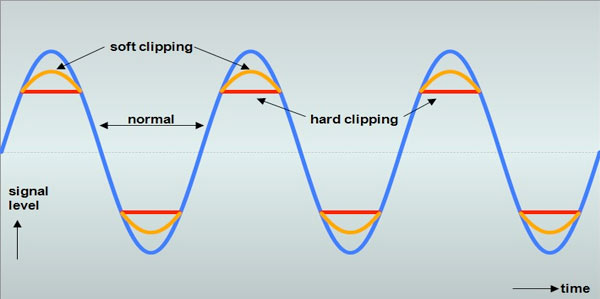
\includegraphics[width=0.8\columnwidth]{immagini/cap2/clipping.jpg}
    \caption{Il fenomeno del Clipping}
\end{figure}

\subsection{Waveshaping}
La tecnica di distorsione del segnale \textit{Waveshaping} viene descritta in modo preciso e puntuale nel libro \textit{The Theory and Technique of Electronic Music}\footcite{puckette:theoryandtechniqueofelectronicmusic} come un passaggio del segnale originale attraverso una funzione non lineare opportunamente scelta. La funzione f(), chiamata \textit{funzione di trasferimento}, distorce la forma d'onda in ingresso in una forma diversa. La nuova forma dipende dalla forma dell'onda in input, dalla funzione di trasferimento e anche, in modo cruciale, dall'ampiezza del segnale in ingresso. Poiché l'ampiezza della forma d'onda in input influenza direttamente la forma della forma d'onda in output (e quindi il timbro), questo dà la possibilità di creare una famiglia di timbri che varia continuamente, semplicemente variando il livello di ingresso della trasformazione. Per questo motivo, è consuetudine includere un controllo di ampiezza iniziale come parte dell'operazione di waveshaping. \\ 
L'ampiezza della forma d'onda in ingresso è chiamata \textit{indice} della forma d'onda. In molte situazioni un indice piccolo porta a una distorsione relativamente piccola (in modo che l'output assomigli molto all'input) e uno più grande dà un timbro più distorto e più ricco. \\
La figura 2.2 mostra un esempio di waveshaping in cui f() equivale a una funzione di clipping. Questo esempio mostra chiaramente come l'indice può influenzare la forma d'onda di output. La funzione di clipping \textbf{(b)} passa il suo input direttamente all'output senza variarlo fintanto che rimane nell'intervallo tra - 0.3 e +0.3. Quindi, quando l'input non supera 0,3 in valore assoluto, l'output è uguale all'input. Tuttavia quando l'input cresce oltre i limiti, l'output viene fatto rimanere entro essi e, all'aumentare dell'ampiezza del segnale, l'effetto di questa azione di clipping diventa progressivamente più importante. Nella figura 2.2 il segnale di input è una sinusoide smorzata \textbf{(a)} e l'output \textbf{(c)} evolve nell'asse x da una forma d'onda quasi quadra all'inizio ad una sinusoide pura alla fine.
\begin{figure}[!h] 
    \centering 
    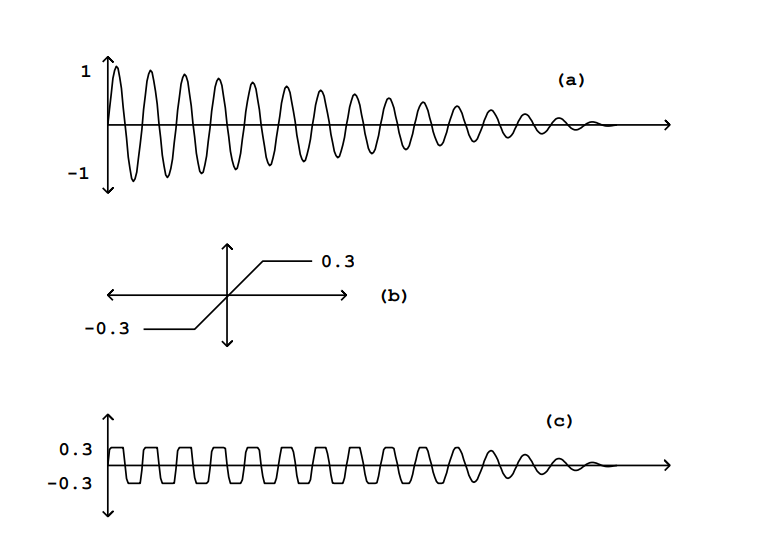
\includegraphics[width=0.8\columnwidth]{immagini/cap2/waveshaper_graph.png}
    \caption{Componenti del Waveshaper}
\end{figure}

\subsection{Bitcrushing}
Il \textit{Bitcrusher} consiste in un processore di segnale che produce distorsione \textit{riducendo la risoluzione dei dati audio digitali}. Gli artefatti introdotti utilizzando questa tecnica possono produrre una sonorità più calda o aspra, a seconda della quantità di degradazione del segnale, andando a simulare il suono prodotto dai vecchi campionatori disponibili all'inizio dell'era digitale. \\
Il bitcrusher utilizza principalmente due metodi per ridurre la fedeltà audio: la riduzione della frequenza di campionamento e la riduzione della profondità di bit.
\begin{itemize}
    \item \textbf{Frequenza di campionamento}: secondo la teoria del campionamento\footcite{burk-polansky-repetto-roberts-rockmore:musicandcomputers}, l'audio digitale è composto da una rapida serie di campioni numerici, acquisiti in modo periodico da un apposito dispositivo chiamato convertitore analogico/digitale, i quali codificano l'ampiezza variabile di una forma d'onda audio. Per una rappresentazione accurata di un segnale audio si necessità di una \textit{frequenza di campionamento} elevata, in quanto maggiore è la frequenza di campionamento, più accurata risulta la forma d'onda. Infatti nel caso in cui il campionamento avvenga ad una frequenza troppo bassa le componenti frequenziali più elevate vengono codificate con troppe poche informazioni e la loro ricostruzione produce degli artefatti. Questo fenomeno, chiamato \textit{aliasing}, avviene nel caso in cui la frequenza di campionamento risulta minore del doppio della frequenza massima del segnale (Teorema del campionamento di Nyquist-Shannon). Sfruttando questo fenomeno il bitcrusher effettua una riduzione graduale, attraverso un apposito parametro, della frequenza di campionamento, introducendo quindi frequenze non armonicamente legate al segnale originale;
    \item \textbf{Profondità di bit}: i singoli campioni nell'audio digitale vengono solitamente registrati come numeri in \textit{virgola mobile} e memorizzati nella memoria digitale utilizzando la \textit{codifica binaria}. In questo modo maggiore è il numero di bit disponibili per rappresentare il livello di ampiezza dei singoli campioni, più accuratamente le forme d'onda vengono campionate. La riduzione della risoluzione effettuata dal bitcrusher riduce intenzionalmente il numero di bit utilizzati per i campioni audio. Man mano che la profondità di bit diminuisce, le forme d'onda diventano più rumorose e si perdono sottili variazioni di volume, riducendo quindi la gamma dinamica. Alla riduzione estrema dei bit a disposizione, le forme d'onda vengono ridotte a delle onde quadre o addirittura a singoli click, aggiungendo quindi molte alte frequenze nello spettro sonoro. 
\end{itemize}
\begin{figure}[!h] 
    \centering 
    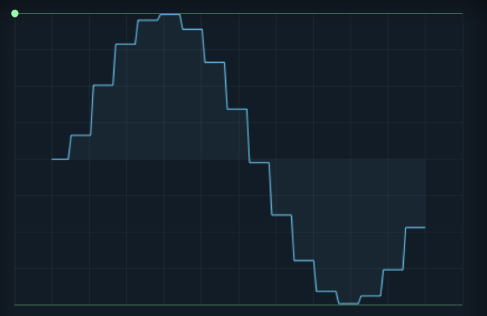
\includegraphics[width=0.8\columnwidth]{immagini/cap2/bitcrusher.png}
    \caption{Riduzione della risoluzione del segnale in un Bitcrusher}
\end{figure}

\subsection{Slew Limiting}
Lo \textit{Slew Limiter} consiste in un processore di segnale audio, solitamente presente come singolo modulo nei sintetizzatori modulari analogici, che permette di livellare un segnale in ingresso in modo che la variazione del livello di tensione non possa superare un certo numero di volt al secondo. Per questo motivo il processore in questione viene solitamente utilizzato come controller di portamento e può essere utilizzato anche come un semplice generatore di inviluppi Attack-Release.\\
Una emulazione digitale di questo particolare processore è implementata nel software Biztortion ed è ispirata al modulo Eurorack \textit{Slew Limiter}\footcite{site:slewlimiter} dell'azienda Befaco, del quale esiste un'implementazione digitale per il software VCV Rack distribuita con \hyperref[cap:licenze-software]{licenza GPL-3.0}. In particolare in questo algoritmo risulta possibile impostare la soglia di velocità massima sopra alla quale essa stessa viene limitata nel tempo sul segnale in uscita, sia nella fase in cui l'onda si muove verso la zona positiva (\textit{Rise}), sia durante la fase in cui l'onda procede nella direzione opposta (\textit{Fall}), andando in questo modo a distorcere la forma d'onda dell'audio.
\begin{figure}[!h] 
    \centering 
    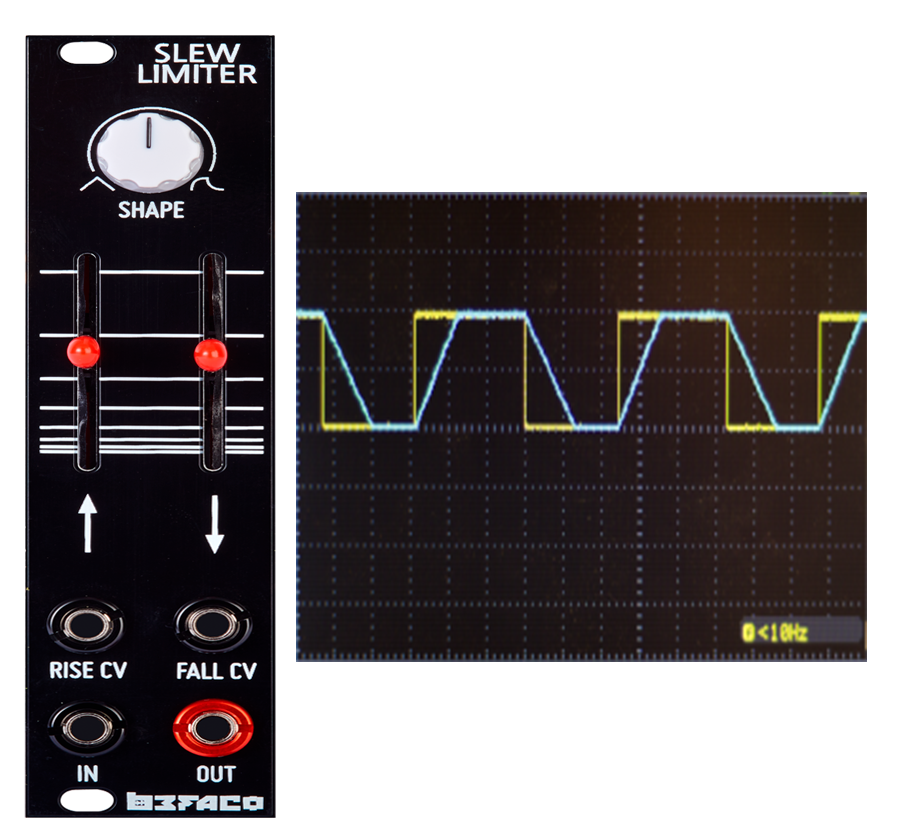
\includegraphics[width=0.8\columnwidth]{immagini/cap2/slew-limiter_Befaco.png}
    \caption{Funzionamento del modulo Slew Limiter dell'azienda Befaco: i segnali in ingresso e uscita sono rispettivamente giallo ed azzurro}
\end{figure}

%**************************************************************
\section{Studio dello stato dell'arte}
In questa sezione viene effettuata un'analisi di alcuni prodotti software presenti sul mercato che offrono diverse tipologie di algoritmi e strumenti utili per la distorsione del segnale audio. \\
Questi prodotti sono stati utilizzati come fonte d'ispirazione per la creazione dell'interfaccia grafica del software \textit{Biztortion}, utili prevalentemente per identificare il layout più funzionale per massimizzare la user experience. Questa ricerca si è rivelata utile inoltre per effettuare un'analisi dei pregi e difetti dei processori di segnale in questione, in modo da poter ricreare nel modo più fedele possibile le funzionalità utili e allo stesso tempo effettuare degli aggiustamenti o aggiunte ad alcuni algoritmi nel software sopraccitato.

\subsection*{Izotope Trash 2}
\noindent \textit{Izotope Trash 2}\footcite{site:trash2} consiste in un processore di segnale audio digitale, disponibile come \gls{pluging} audio in diversi formati, che consente una trasformazione sonora complessa grazie alla presenza di un elevato numero di moduli che offrono diverse funzionalità.
%\clearpage
\begin{figure}[!h] 
    \centering 
    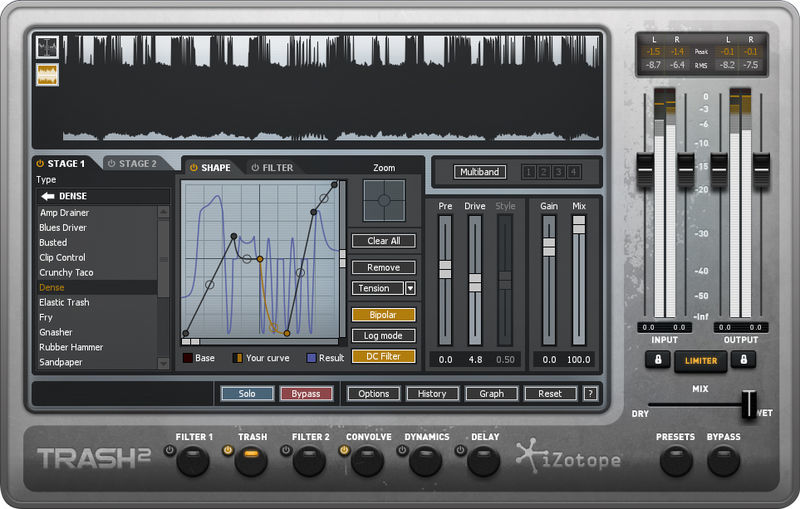
\includegraphics[width=0.8\columnwidth]{immagini/cap2/trash2.jpg}
    \caption{Izotope Trash 2}
\end{figure} \\
I moduli offerti dal software sono i seguenti:
\begin{itemize}
    \item \textbf{Pre/Post-filtering}: i moduli per il filtraggio del segnale consentono di modellare lo spettro sonoro utilizzando fino a 6 filtri, i quali possono essere configurati con oltre 20 modelli differenti. Sono inoltre utilizzabili degli \gls{lfog}, inviluppi e il \gls{sidechaing} per la modulazione dei parametri;
    \item \textbf{Trash}: il modulo in questione consente la distorsione del segnale utilizzando oltre 60 funzioni di trasferimento per effettuare waveshaping in due stadi, con la possibilità di applicare l'effetto a tutto lo spettro o fino a 4 bande di frequenze differenti;
    \item \textbf{Convolve}: attraverso il modulo per la convoluzione del segnale Trash 2 consente una simulazione realistica di diversi altoparlanti ed acustiche, permettendo di posizionare completamente l'audio in un altro luogo o oggetto;
    \item \textbf{Dynamics}: consente la compressione multibanda del segnale utilizzando fino a 4 bande di frequenze differenti;
    \item \textbf{Delay}: consente l'aggiunta dell'effetto Echo offrendo fino a 6 algoritmi diversi.
\end{itemize}

\subsection*{Kilohearts Toolbox}
\noindent \textit{Kilohearts Toolbox}\footcite{site:toolbox} consiste in un pacchetto, del quale esistono diverse versioni in base al budget che si vuole investire nel suo acquisto, che offre vari strumenti che fanno parte dell'ecosistema Kilohearts. In questo pacchetto sono compresi diversi \gls{pluging} audio, utilizzabili singolarmente all'interno della \gls{dawg} desiderata, e l'host di effetti modulari gratuito, Snap Heap, per poter combinare i singoli \gls{pluging} in rack di effetti seriali e/o paralleli. \\
\begin{figure}[!h] 
    \centering 
    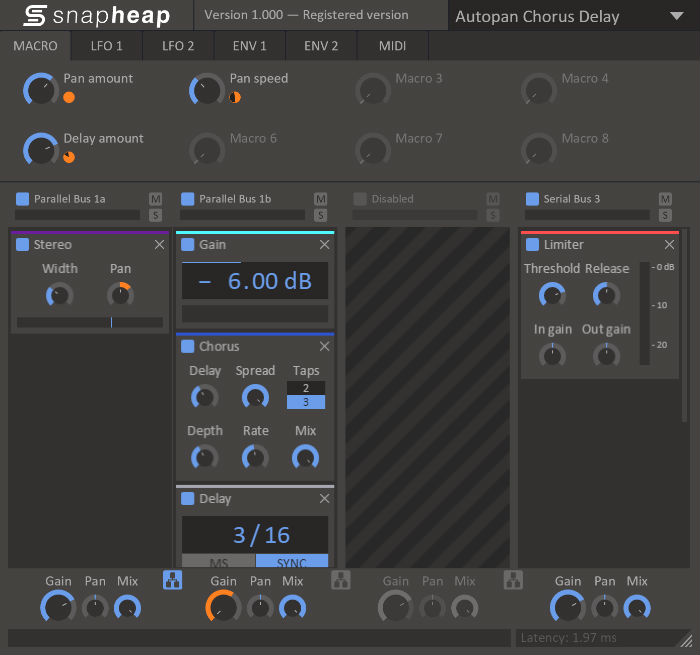
\includegraphics[width=0.8\columnwidth]{immagini/cap2/kilohearts.jpg}
    \caption{Kilohearts Snap Heap}
\end{figure} \\
Tra l'elevato numero di effetti presenti nel pacchetto in questione sono compresi i seguenti \gls{pluging} che effettuano la distorsione del segnale:
\begin{itemize}
    \item \textbf{Distortion}: consiste in un processore di segnale in cui è possibile utilizzare 5 diversi algoritmi, i quali utilizzano diverse combinazioni di waveshaping e filtri, per la distorsione dell'audio in ingresso. Risulta inoltre possibile aggiungere un DC offset al segnale prima del processing e, utilizzando un apposito potenziometro, differenziare l'offset stesso tra i due canali sinistro e destro, in modo da creare dei sottili ampliamenti della stereofonia;
    \item \textbf{Bitcrush}: permette di simulare l'audio come se fosse riprodotto utilizzando un campionatore di bassa qualità, con frequenza di campionamento e profondità di bit limitate. Questo processore di segnale consente inoltre l'aggiunta di rumore in modo effettuare del \gls{ditheringg} per ridurre il rumore causato dalla quantizzazione, oltre all'utilizzo di appositi filtri per la diminuzione dell'aliasing causato dalla riduzione della qualità del campionamento (sia ad alte che basse frequenze);
    \item \textbf{Phase Distortion}: consiste in un processore audio che consente al segnale di modulare la fase di se stesso, risultando sostanzialmente in qualcosa di simile al feedback FM. Questo effetto infatti non modifica l'ampiezza del segnale, come effettuano invece i distorsori tradizionali, ma trasforma la fase di singole armoniche usando l'input stesso come modulante. Poichè l'input influenza direttamente l'algoritmo per la produzione del segnale in uscita, l'effetto risultante è sempre originale e non può suonare uguale in due moduli diversi.
\end{itemize}

% TODO : aggiungo paragrafo con descrizione Fabfilter Saturn

\subsection*{Fabfilter Saturn 2}
\noindent \textit{Fabfilter Saturn 2}\footcite{site:saturn2} consiste in un processore di segnale audio digitale, disponibile come \gls{pluging} audio in diversi formati, che offre una vasta gamma di algoritmi di distorsione ispirati al mondo analogico vintage degli amplificatori a valvole e dei nastri magnetici. Sono inoltre presenti diversi algoritmi basati su differenti tecniche di distorsione come il bitcrushing o la granularizzazione del segnale. 
\begin{figure}[!h] 
    \centering 
    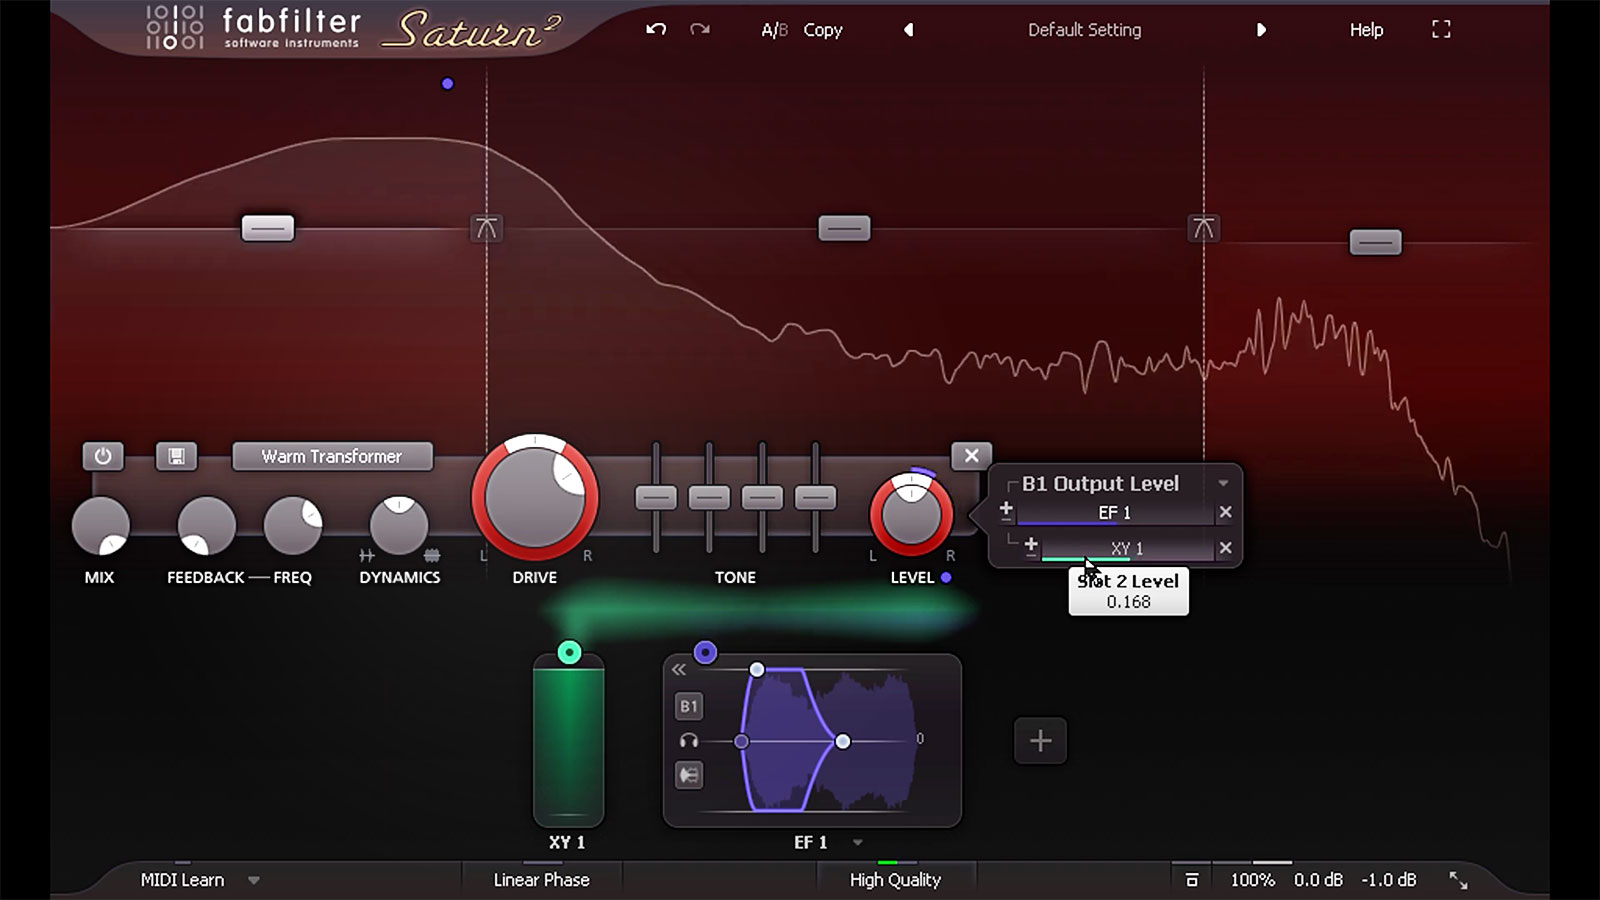
\includegraphics[width=0.8\columnwidth]{immagini/cap2/saturn2.jpg}
    \caption{Fabfilter Saturn 2}
\end{figure} \\
Le funzionalità salienti del software sono le seguenti:
\begin{itemize}
    \item \textbf{Display multibanda interattivo}: il display interattivo consente di creare e selezionare direttamente le bande di frequenza e, allo stesso tempo, è un analizzatore di frequenza in tempo reale, permettendo di visualizzare il segnale in uscita e rendendo facile decidere dove impostare le frequenze di crossover della banda;
    \item \textbf{Controlli delle bande}: i controlli delle bande controllano le impostazioni delle bande selezionate nel display. Per ogni banda, è possibile regolare separatamente il tipo di distorsione, il drive, le impostazioni di feedback, le dinamiche, il tono, il livello e le impostazioni di mix;
    \item \textbf{Sezione di modulazione}: la sezione di modulazione, presente nella parte inferiore dell'interfaccia mostra tutte le sorgenti disponibili per la modulazione dei parametri, ovvero  \gls{lfog}, envelope generator (EG), envelope follower (EF), controller MIDI e XY;
    \item \textbf{Fase lineare}: quando la modalità "Linear Phase" è abilitata, sia il filtro crossover multibanda che l'oversampling interno, attivabile attraverso la modalità "High Quality", vengono eseguiti utilizzando un filtraggio a fase lineare.
\end{itemize}             % Distorsione
% !TEX encoding = UTF-8
% !TEX TS-program = pdflatex
% !TEX root = ../tesi.tex

%**************************************************************
\chapter{Descrizione dello stage}
\label{cap:descrizione-stage}
%**************************************************************

\intro{Breve introduzione al capitolo}\\

%**************************************************************
\section{Introduzione al progetto}

%**************************************************************
\section{Analisi preventiva dei rischi}

Durante la fase di analisi iniziale sono stati individuati alcuni possibili rischi a cui si potrà andare incontro.
Si è quindi proceduto a elaborare delle possibili soluzioni per far fronte a tali rischi.\\

\begin{risk}{Performance del simulatore hardware}
    \riskdescription{le performance del simulatore hardware e la comunicazione con questo potrebbero risultare lenti o non abbastanza buoni da causare il fallimento dei test}
    \risksolution{coinvolgimento del responsabile a capo del progetto relativo il simulatore hardware}
    \label{risk:hardware-simulator} 
\end{risk}

%**************************************************************
\section{Requisiti e obiettivi}


%**************************************************************
\section{Pianificazione}             % Biztortion
% !TEX encoding = UTF-8
% !TEX TS-program = pdflatex
% !TEX root = ../tesi.tex

%**************************************************************
\chapter{Licenze software}
\label{cap:licenze-software}
%**************************************************************

\intro{Il capitolo in questione effettua una panoramica sulle licenze per il software libero, analizzando quelle utilizzate dalle librerie terze necessarie all'implementazione del software Biztortion e quindi quella utilizzata per il rilascio del suddetto software}\\

%**************************************************************
\section{Software libero}

Il software \hyperref[cap:biztortion]{Biztortion}, corrispondente a parte del lavoro effettuato per la tesi di laurea, è stato sviluppato con l'obiettivo di approfondire il fenomeno della distorsione del segnale audio e di aumentare il mio bagaglio di esperienza da programmatore. Essendo inoltre la tesi di laurea un lavoro di studio e ricerca, risuta logicamente ed eticamente corretto il rilascio e la diffusione del software in questione come \textit{software libero}. \\ \\
Il “Software libero”\footcite{site:software-libero} rispetta la libertà degli utenti e la comunità. In breve, significa che gli utenti hanno la libertà di eseguire, copiare, distribuire, studiare, modificare e migliorare il software. Tramite queste libertà gli utenti (individualmente o nel loro complesso) controllano il programma e le sue funzioni. Quando non sono gli utenti a controllare il programma, allora il programma (che in quel caso è denominato "non libero" o "proprietario") controlla gli utenti. \\
Un programma è software libero se gli utenti del programma godono delle quattro libertà fondamentali:
\begin{enumerate}
    \item Libertà di \textbf{eseguire} il programma come si desidera, per qualsiasi scopo;
    \item Libertà di \textbf{studiare} come funziona il programma e di \textbf{modificarlo} in modo da adattarlo alle proprie necessità. L'accesso al codice sorgente ne è un prerequisito;
    \item Libertà di \textbf{ridistribuire} copie in modo da aiutare gli altri;
    \item Libertà di \textbf{migliorare} il programma e distribuirne pubblicamente i miglioramenti apportati (e le versioni modificate in genere), in modo tale che tutta la comunità ne tragga beneficio. Anche qui l'accesso al codice sorgente ne è un prerequisito.
\end{enumerate}
E' necessario inoltre evidenziare il fatto che software libero non vuol dire non commerciale. Al contrario, con un programma libero deve essere possibile anche l'\textbf{uso commerciale}, lo sviluppo commerciale, e la distribuzione commerciale. Questa politica è di importanza fondamentale, infatti senza questa il software libero non potrebbe raggiungere i suoi obiettivi. \\
Infine certi tipi di regole sul come distribuire il software libero sono accettabili quando non entrano in conflitto con le libertà principali. Per esempio, il \textbf{copyleft}, noto anche impropriamente come "permesso d'autore", è in poche parole la regola per cui, quando il programma è ridistribuito, non è possibile aggiungere restrizioni per negare ad altre persone le libertà principali. Questa regola non entra in conflitto con le libertà principali, anzi le protegge.

%**************************************************************
\section{Licenze per il software libero}
Una licenza di software libero è una licenza libera, un testo legale caratterizzato da un aspetto contrattuale o para-contrattuale, che si applica ad un software per garantirne la libertà d'utilizzo, di studio, di modifica e di condivisione, ovvero per renderlo software libero. \\
La nascita del concetto di licenza applicata ad un software per renderlo libero combacia in parte con la nascita di \textit{GNU}, il primo sistema operativo completamente libero ideato da Richard Stallman nel 1983. Tutt'oggi il progetto GNU e la Free Software Foundation patrocinano attivamente il software distribuito sotto licenze libere e, in generale, la libertà digitale degli utenti. \\ \\
Di seguito vengono descritte alcune tra le licenze per il software libero utilizzate dalle librerie esterne necessarie allo sviluppo del software \textit{Biztortion}.

\subsection{GPL}
\label{sec:gpl}
La \textit{GNU General Public License}\footcite{site:gpl} (comunemente indicata con l'acronimo GNU GPL o semplicemente GPL) è una licenza \textit{fortemente copyleft} per software libero, originariamente stesa nel 1989 da Richard Stallman per patrocinare i programmi creati per il sistema operativo GNU. \\
La Free Software Foundation (FSF) detiene i diritti di copyright sul testo della GNU GPL, ma non detiene alcun diritto sul software da essa coperto. La GNU GPL non è liberamente modificabile: solo la copia e la distribuzione sono permesse. Per questo motivo solo la FSF può pubblicare nuove revisioni o versioni, l'ultima delle quali fu pubblicata il 29 giugno del 2007 sotto il nome di \textbf{GNU GPL v3}.

\subsection{MIT}
La \textit{Licenza MIT}\footcite{site:mit} è una licenza di software libero creata dal Massachusetts Institute of Technology (MIT). 
La licenza in questione è \textit{senza copyleft} e risulta molto permissiva, in quanto a differenza delle licenze software copyleft, la licenza MIT consente anche il riutilizzo all'interno di software proprietario, a condizione che tutte le copie del software o delle sue parti sostanziali includano una copia dei termini della licenza MIT e anche un avviso di copyright. La licenza MIT È anche una licenza \textit{GPL-compatibile}, cioè la GPL permette di combinare e ridistribuire tale software con altro che usa la licenza MIT.

\subsection{BSD}
Le \textit{licenze BSD} sono una famiglia di licenze permissive, \textit{senza copyleft}, per software libero. Il loro nome deriva dal fatto che la licenza BSD originale (detta anche licenza BSD con 4 clausole) fu usata originariamente per distribuire il sistema operativo Unix Berkeley Software Distribution (BSD), una revisione libera di UNIX sviluppata presso l'Università di Berkeley. \\
La versione originale è stata successivamente rivista e le sue discendenti sono più propriamente definite licenze BSD modificate. Due varianti della licenza, la Nuova Licenza BSD (o Licenza BSD Modificata)\footcite{site:bsd} e la Licenza semplificata BSD (o FreeBSD), sono state verificate come licenze di software libero \textit{GPL-compatible} dalla Free Software Foundation.

%**************************************************************
\section{Librerie utilizzate}
Per la realizzazione del software \textit{Biztortion} sono state utilizzate delle librerie sviluppate da terzi in modo da semplificare lo sviluppo di alcuni componenti. Di seguito vengono elencate e descritte tutte le librerie in questione, le quali utilizzano tutte delle licenze per software libero che sono \textit{GPL-compatible} rendendo più semplice la scelta della licenza di rilascio e distribuzione del software sopraccitato:
\begin{itemize}
    \item \textbf{JUCE}: il framework C++ in questione, necessario per la creazione dell'applicazione audio, utilizza termini di licenza a vari livelli, con termini diversi per ogni licenza disponibile: \textit{JUCE Personal} (per sviluppatori o start-up con entrate inferiori al limite di entrate di 50K USD; gratuito), \textit{JUCE Indie} (per le piccole imprese con limite di entrate inferiore a 500K USD; \$ 40/mese), \textit{JUCE Pro} (nessun limite di entrate; \$ 130/mese) e \textit{JUCE Educational} (nessun limite di entrate; gratuito per istituzioni educative in buona fede). Risulta infine possibile rilasciare un'applicazione sviluppata con JUCE sotto la \textbf{GNU GPLv.3}, rendendola software libero in modo che ne possa beneficiare tutta la comunità;
    \item \textbf{dRowAudio}: consiste in un modulo JUCE di terze parti progettato per lo sviluppo rapido di applicazioni audio; la libreria, sviluppata da \textit{David Rowland}, contiene diverse classi per l'elaborazione audio e vari elementi utili per la creazione dell'interfaccia grafica. Il modulo in questione è distribuito secondo i termini della \textbf{Licenza MIT} per il software libero;
    \item \textbf{ff\_meters}: consiste in un modulo JUCE di terze parti che offre un componente facile da usare per visualizzare una lettura di livello del segnale utilizzando un \textit{juce::AudioBuffer} in ingresso. La libreria, sviluppata da \textit{Daniel Walz} (Foleys Finest Audio Ltd.), deve essere utilizzata con il framework JUCE. Il modulo in questione è distribuito secondo i termini della \textbf{Licenza BSD a 3 clausole} (conosciuta anche come "Nuova" o "Modificata").
\end{itemize}

%**************************************************************
\section{Software Biztortion}
Il software \textit{Biztortion}, poiché è stato sviluppato con le librerie citate nella sezione precedente che utilizzano licenze per il software libero \textit{GPL-compatible}, viene distribuito secondo i termini stabiliti dalla licenza \hyperref[sec:gpl]{GNU GPLv.3}, ovvero la più recente delle GPL. In sostanza la licenza in questione, oltre ad affermare le quattro libertà fondamentali del software libero, garantisce che tutte le versioni migliorate a partire da quella originale che saranno distribuite dovranno essere libere a loro volta. \\ \\
Il software in questione viene rilasciato, insieme al presente documento per la discussione della tesi di laurea, alla versione \textit{1.0} ed è possibile trovare tutti i file corrispondenti al prodotto software in \href{https://github.com/killbizz/Biztortion}{questo repository remoto}.             % Licenze
% !TEX encoding = UTF-8
% !TEX TS-program = pdflatex
% !TEX root = ../tesi.tex

%**************************************************************
\chapter{Conclusioni}
\label{cap:conclusioni}
%**************************************************************
\section{Analisi del lavoro svolto}
Il lavoro necessario alla realizzazione della tesi di laurea è risultato molto interessante e stimolante. La prima parte di esso, prevedendo uno studio sul fenomeno della distorsione del segnale audio, mi ha permesso di approfondire un concetto creativamente molto importante, in modo tale da poterlo applicare con criterio nell'implementazione degli algoritmi presenti nel software \textit{Biztortion}. \\
La realizzazione del software in questione è risultata la parte più entusiasmante in quanto ha permesso di acquisire a livello pratico nuove abilità e competenze, oltre a consolidare quelle già possedute. \\
Il mio percorso di studi è risultato fondamentale per un corretto sviluppo del \gls{pluging} audio; infatti il mio background accademico mi ha fornito le conoscenze di base legate all'\textit{informatica musicale} (come per esempio l'audio digitale, il \gls{dspg} e i filtri digitali) necessarie per un corretto approccio all'audio programming. Inoltre la mia carriera universitaria, legata alle scienze informatiche, ha reso possibile una buona analisi del problema e progettazione del software ancora prima di iniziare la fase di codifica, oltre che ad un rapido apprendimento autonomo delle tecnologie necessarie allo sviluppo del \gls{pluging} stesso. In particolare ho potuto apprezzare una certa rapidità di scrittura del codice grazie all'esperienza con la programmazione ad oggetti e con il linguaggio di programmazione C++, maturata durante il corso universitario di \textit{Programmazione ad Oggetti}. Un ulteriore merito va dato inoltre al corso universitario di \textit{Ingegneria del Software}, il quale mi ha dato le competenze necessarie ad una gestione efficiente ed efficace di un progetto software, oltre alla conoscenza degli strumenti legati alla stesura del presente documento.

%**************************************************************
\section{Conoscenze acquisite}
Lo sviluppo del software \textit{Biztortion} mi ha permesso di interfacciarmi per la prima volta con il mondo della programmazione per l'audio, consentendomi di imparare in modo rapido e molto concreto alcune \textit{tecnologie} ad asso legate come i formati VST/AU e il framework JUCE, il quale risulta molto popolare e utile anche per iniziare una carriera nel relativo ambito lavorativo. \\
Inoltre entrando nell'ottica dell'audio programming ho avuto la possibilità di \textit{comprendere meglio le problematiche} legate a questa professione: in particolare ho verificato in prima persona l'impatto che le performance fornite sia dall'hardware che dal software hanno con la produzione del suono, rendendole fondamentali sia per l'elaborazione del segnale audio in tempo reale che per semplicemente evitare che le strumentazioni analogiche si possano danneggiare a causa di una produzione di click nell'audio in uscita. \\
Infine è stato molto interessante l'approfondimento effettuato sulle \textit{licenze software} e sulle tecnologie \gls{opensourceg}, risultate come uno strumento molto potente e di fondamentale importanza per tutti gli sviluppatori in modo tale che possano dare valore aggiunto all'intera community.

%**************************************************************
\section{Valutazione personale}
In conclusione ritengo che questo periodo, dedicato al lavoro per la tesi di laurea, mi abbia permesso di conoscere meglio e migliorare le mie capacità informatiche e di gestione delle tempistiche in modo autonomo. \\
Il lavoro svolto è stato molto interessante, stimolante ed appagante in quanto mi ha permesso un primo assaggio della parte tecnica del lavoro di un \textit{audio programmer}, motivandomi ulteriormente nel cercare di cominciare una carriera in questo ambito lavorativo.             % Conclusioni
%\appendix                               
%% !TEX encoding = UTF-8
% !TEX TS-program = pdflatex
% !TEX root = ../tesi.tex

%**************************************************************
\chapter{Appendice A}
%**************************************************************

\epigraph{Citazione}{Autore della citazione}



             % Appendice A

%**************************************************************
% Materiale finale
%**************************************************************
\backmatter
\printglossaries
% !TEX encoding = UTF-8
% !TEX TS-program = pdflatex
% !TEX root = ../tesi.tex

%**************************************************************
% Bibliografia
%**************************************************************

\cleardoublepage
\chapter{Bibliografia}

\nocite{*}
% Stampa i riferimenti bibliografici
\printbibliography[heading=subbibliography,title={Riferimenti bibliografici},type=book]

% Stampa i siti web consultati
\printbibliography[heading=subbibliography,title={Siti web consultati},type=online]


\end{document}
